\subsection{Visão geral do GenBank-NCBI no All Resources}


\subsubsection{Mycobacterium tuberculosis}

Observar as grandes divisões: Databases, Download, Submission,  Tools, How To. Fazer uma busca em “All Databases” para a espécie Mycobacterium tuberculosis (MTB).  
Listar para cada o maior número possível de seções dos hits mais atuais.

\subsubsubsection{O livro específico para MTB mais atual publicado}
    
\begin{figure}[!htp]
    \centering
    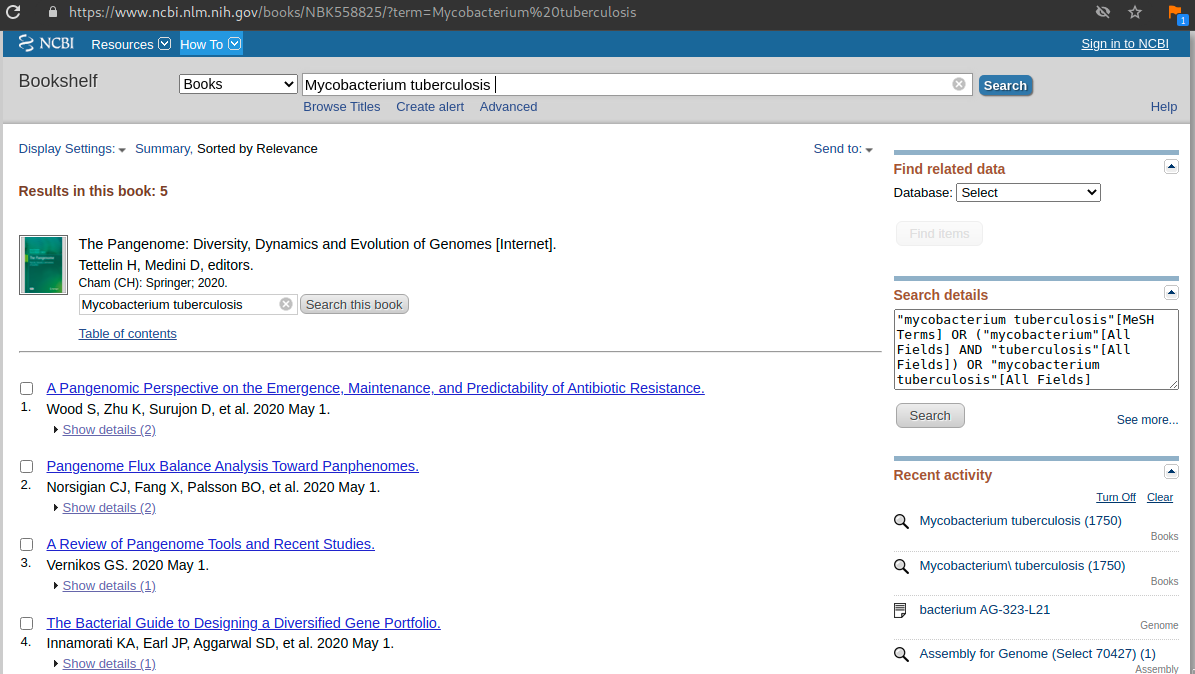
\includegraphics[scale=.37]{img/book.png}
    \caption{Livro mais recente sobre a espécie Mycobacterium tuberculosis é de \citeonline{tettelin2020} }
    \label{img:mtb.book}
\end{figure}

% \footnote{https://www.ncbi.nlm.nih.gov/books/NBK558825/?term=Mycobacterium\%20tuberculosis}
    
    
\newpage    
\subsubsubsection{O artigo em Pubmed específico para tuberculosis mais atual publicado:}

\begin{figure}[!htp]
    \centering
    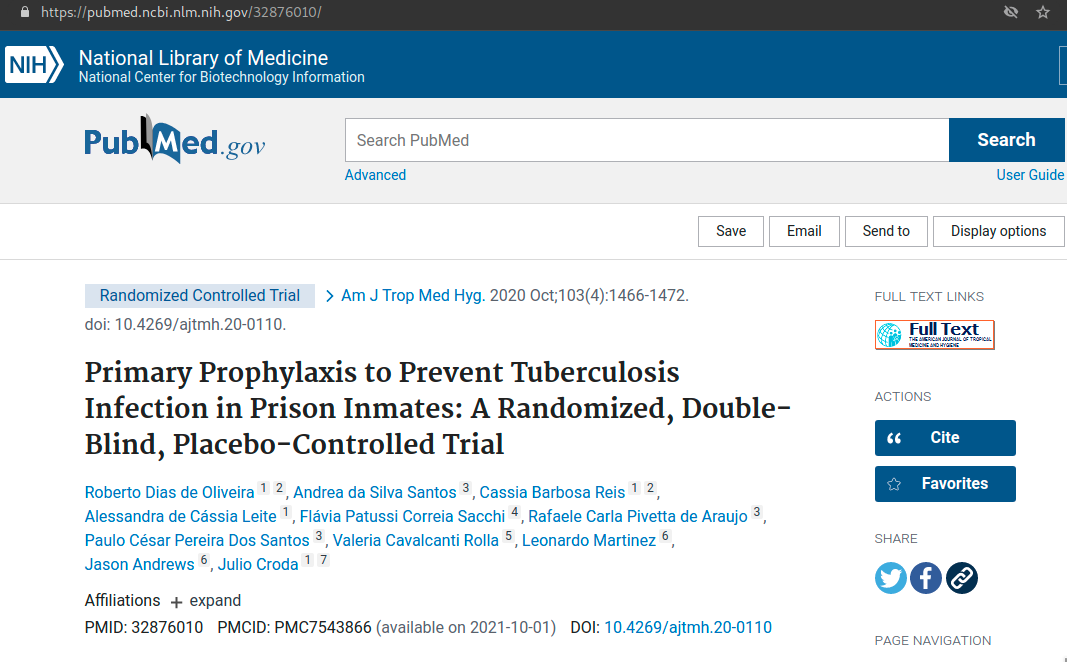
\includegraphics[scale=.38]{img/article.png}
    \caption{Artigo mais recente sobre a espécie Mycobacterium tuberculosis é de \citeonline{Oliveira2020} }
    \label{img:mtb.article}
\end{figure}

% \footnote{https://pubmed.ncbi.nlm.nih.gov/32876010/}:

% Mycobacterium+tuberculosis
% \&filter=simsearch3.fft
% \&filter=pubt.randomizedcontrolledtrial

% \&filter=dates.2020
% \%2F6
% \%2F1-2021
% \%2F1
% \%2F20
% \&ac=no\&sort=date


\subsubsubsection{Quantas em PubmedCentral}

\begin{figure}[!htp]
    \centering
    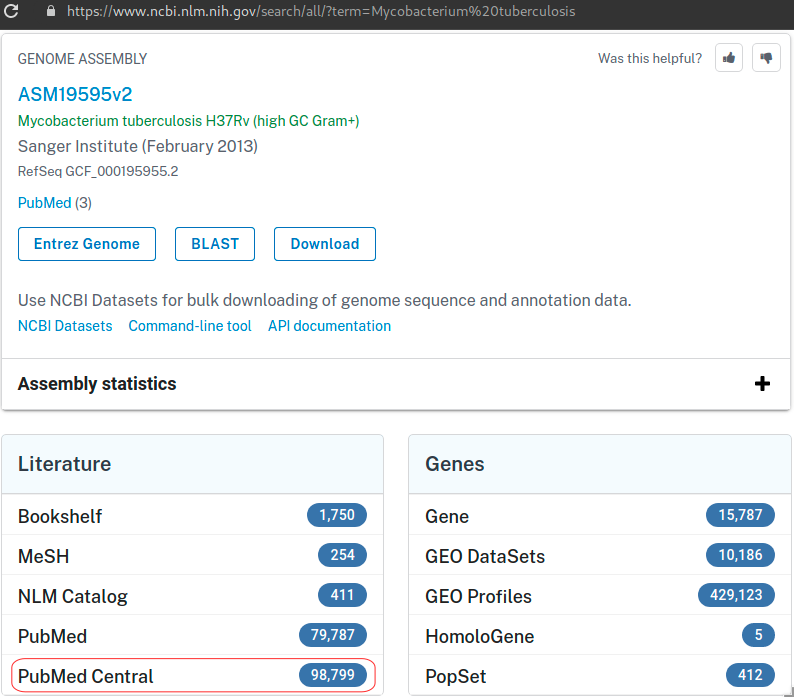
\includegraphics[scale=.385]{img/pubmed_central.png}
    \caption{Existem 98799 resultados em PubMed Central sobre a espécie Mycobacterium tuberculosis}
    \label{img:mtb.pubmed_central}
\end{figure}



\newpage
\subsubsubsection{Qual a entrada nucleotide sequences de M. tuberculosis mais atual depositada} 

Observando a página da seção no menu direita. 
Results by táxon Organisms  [Tree] Mycobacterium tuberculosis.


\begin{figure}[!htp]
    \centering
    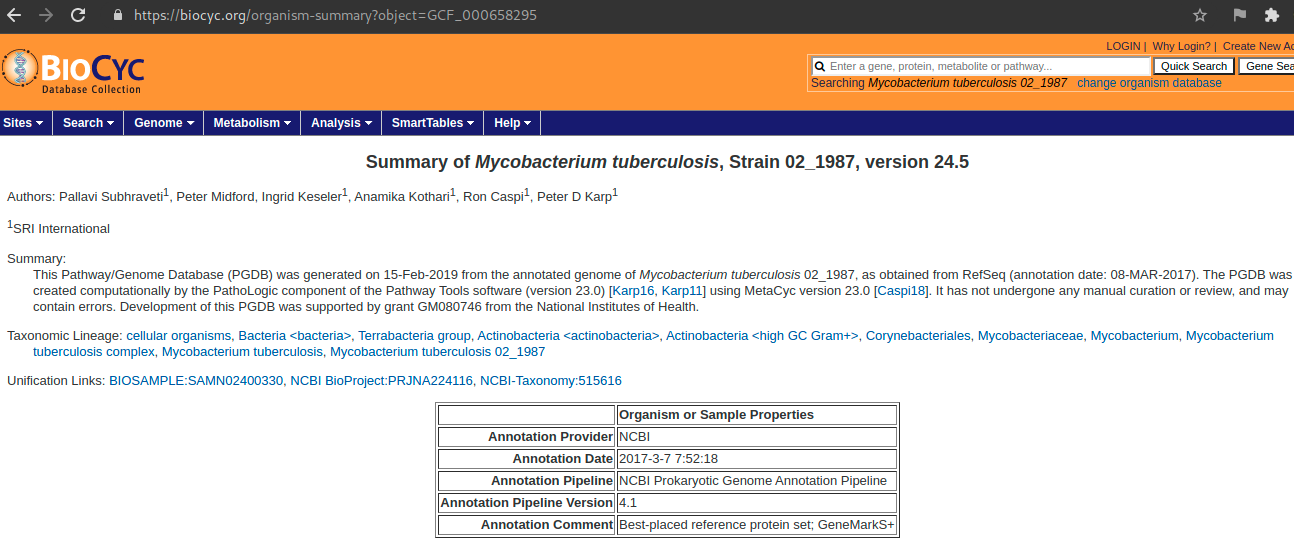
\includegraphics[scale=.35]{img/mtb2017.png}
    \caption{O nucleotide sequences mais recente Mycobacterium tuberculosis 02\underline{\hspace{.1in}}1987 atualizado em 2017}
    \label{img:mtb.nucleotide}
\end{figure}


% O último registro encontrado é de 2017, denominado "Summary of Mycobacterium tuberculosis, Strain 02\underline{\hspace{.1in}}1987, version 24.5" \footnote{https://biocyc.org/organism-summary?object=GCF\underline{\hspace{.1in}}000658295}



\subsubsection{BioProject e BioSample}

O BioProject conjunto de dados biológicos relacionados a uma única iniciativa, oriundos de uma única organização ou consórcio.
O BioSample é um banco de dados que contém descrições de materiais de origem biológica usados em ensaios experimentais.
Portanto, para identificar as entradas para o vírus \textit{SARS-CoV-2} o BioProject disponibiliza 469 resultados
Já o  BioSample 231361 resultados, ambas as pesquisas realizadas no dia 21/01/2020.
A diferença é dada pelo critério de armazenamento do banco de dados biológicos.
Sendo o BioProject mantido pelas organizações, já BioSample armazena ensaios experimentais.
Então, se o número de ensaios é maior que o número de organizações.
Além disso, uma organização pode realizar diversos ensaios experimentais. 


\newpage
\subsubsection{Genome}

Esta seção organiza informações sobre genomas, incluindo sequências, mapas, cromossomos, montagens e anotações.
A divisão dos genomas é representada na Figura~\ref{img:genomas}.


\begin{figure}[!htp]
    \centering
    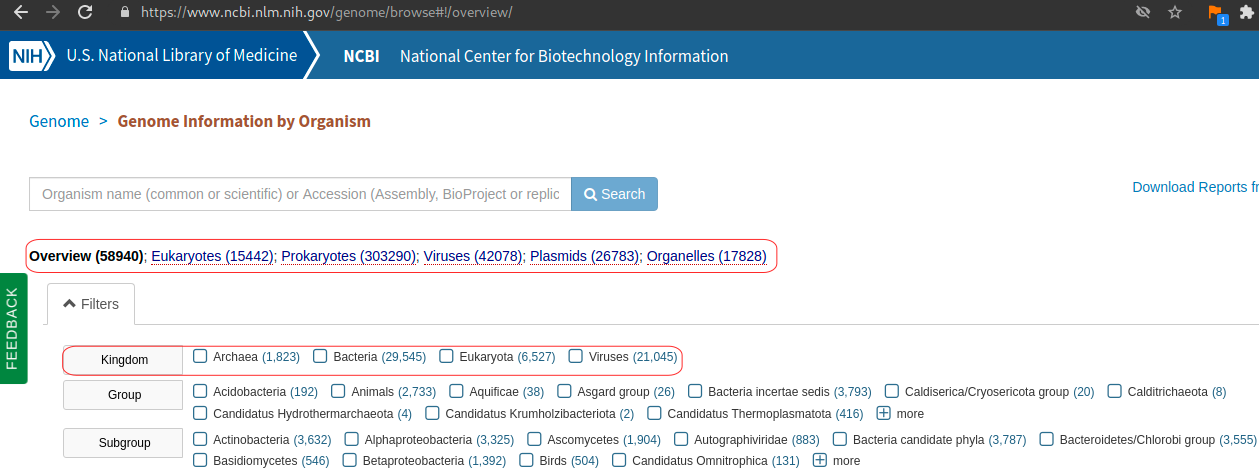
\includegraphics[scale=.36]{img/genome.png}
    \caption{
        Número de genomas são divididos entre a Eucariotas~(15442);  Procarionte~(303290); Vírus~(42078); Plasmídeo~(26783); e Organelas~(17828).
        Além da Kingdom de bactérias que contêm 29545.
    } 
    \label{img:genomas}
\end{figure}


\begin{figure}[!htp]
    \centering
    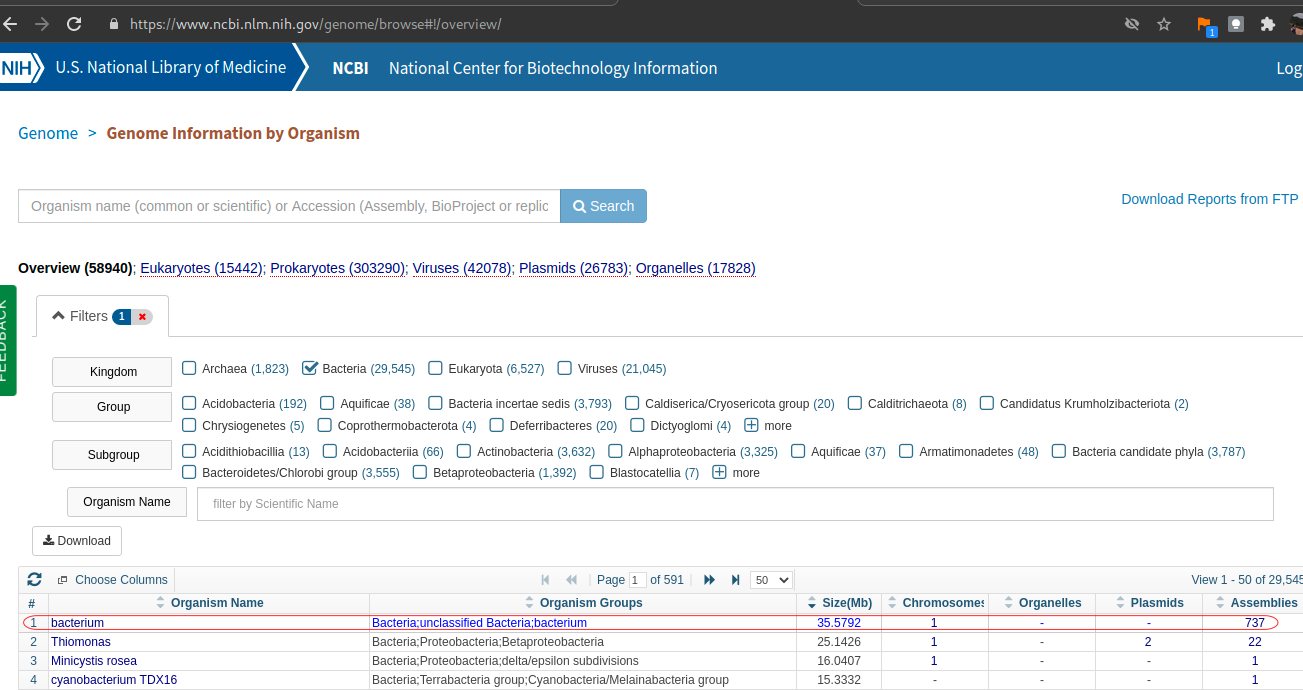
\includegraphics[scale=.33]{img/big_bacterium.png}
    \caption{
        O maior genoma entre as bactérias é a Bacterium
    } 
    \label{img:genomas_bacterium_big}
\end{figure}


\begin{figure}[!htp]
    \centering
    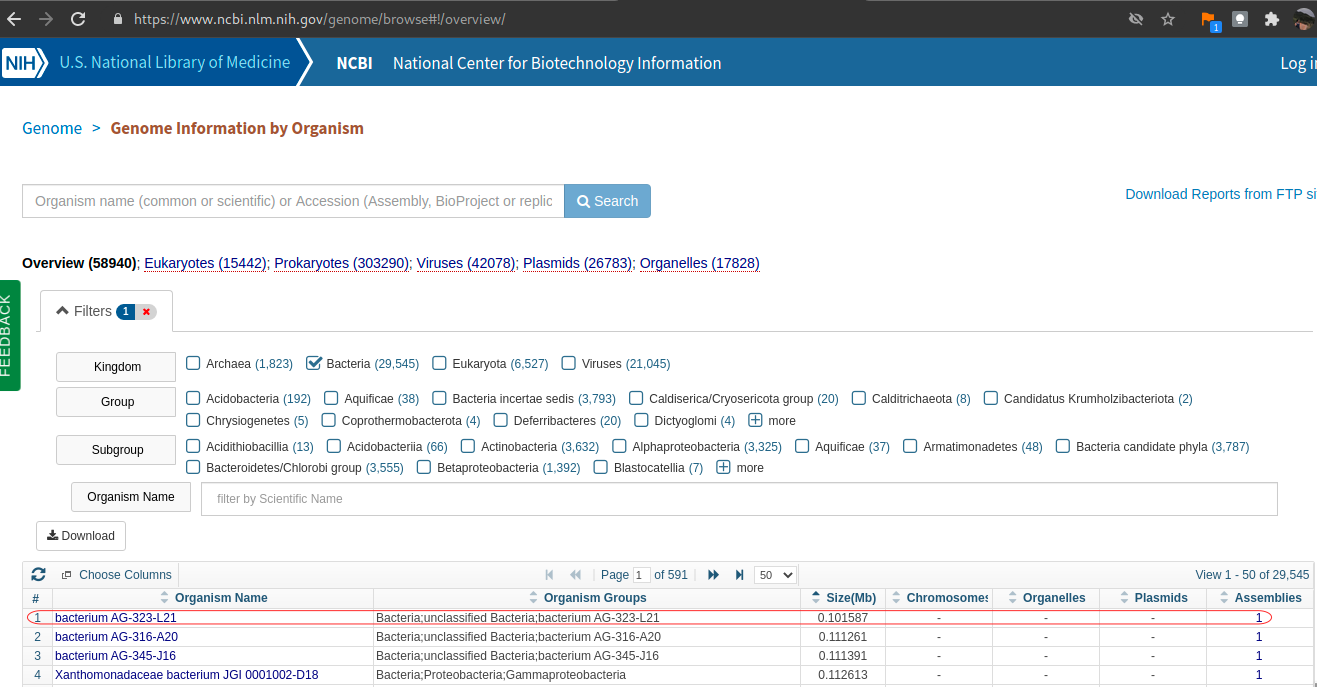
\includegraphics[scale=.33]{img/small_bacterium.png}
    \caption{
        O menor genoma entre as bactérias é a Bacterium
    } 
    \label{img:genomas_bacterium_small}
\end{figure}


% A bactérica que possui o maior genoma é a Bacterium\footnote{https://www.ncbi.nlm.nih.gov/genome/59683} tendo 35.5792~Mb e a menor a Bacterium~AG-323-L21\footnote{https://www.ncbi.nlm.nih.gov/genome/70427} tendo 0.101587~Mb.


\newpage
\subsubsection{PubMed}

Na seção PubMed que inclui links para artigos completos e outras fontes relacionadas. 
O NCBI oferece você criar uma conta pessoal através do MyNCBI, um recurso de utilidade para poder salvar qualquer busca no banco. 

\begin{itemize}
    \item Fazer uma busca cruzando cada um dos termos agr (D, B, C ou A) com Staphylococcus aureus e  identificar quantos artigos foram achados em cada busca.
\end{itemize}


\subsubsection{Taxonomy}
\label{section:taxonomy}

Na seção Taxonomy: Procurar as Sequências de genes agrD, agrB, agrC e agrA em Staphylococcus aureus. 
Para isso iniciar a busca da espécie no Taxonomy browser e depois localizar na tabela “Entrez records” em Direct link: em Nucleotide. 

\begin{itemize}
    \item quantas entradas são recuperadas para cada busca? 
\end{itemize}


\subsubsection{GenBank}
Na seção GenBank. 
GenBank Submission Types: descrever os tipos de submissões permitidas. 
Em Submission tools: investigar como submeter uma Sequência de nucleotídeos no GenBank.

A submissão para o GenBank é aceita em mRNA ou dados de sequência genômica determinados diretamente pelo solicitante. 
O envio deve incluir informações sobre o organismo de origem e anotações fornecidas pelo remetente\footnote{https://www.ncbi.nlm.nih.gov/genbank/submit\underline{\hspace{.1in}}types/}.